\documentclass{amsart}

\usepackage[notref,notcite]{showkeys}
\usepackage[style=authoryear,ibidtracker=false,uniquename=false,giveninits=true,terseinits=true,maxbibnames=5,backend=biber]{biblatex}
\usepackage{float}
\usepackage{graphicx}
\usepackage{todonotes}
\usepackage{subcaption}
\usepackage{amsmath}
\usepackage{amsthm}
\usepackage{amssymb}
\usepackage[foot]{amsaddr}
\usepackage[misc]{ifsym}

\renewbibmacro{in:}{}
\addbibresource{rnni_polynomial.bib}

\newtheorem{lemma}{Lemma}
\newtheorem{theorem}{Theorem}

\newcommand{\rnni}{\mathrm{RNNI}}
\newcommand{\findpath}{\textsc{FindPath}}
\newcommand{\mrca}{\mathrm{mrca}}
\newcommand{\rank}{\mathrm{rank}}
\newcommand{\nni}{\mathrm{NNI}}
\newcommand{\fp}{\mathrm{FP}}
\renewcommand{\O}{\mathcal O}

\graphicspath{{figures/}}


\title[Computing $\rnni$ distance]{Efficient algorithm for computing nearest neighbour interchange distance between ranked phylogenetic trees}
\date{\today}
\author{Lena Collienne\textsuperscript{1}}
\email{lena.collienne@postgrad.otago.ac.nz}
\address{\textsuperscript{1}Department of Computer Science, University of Otago, New Zealand}
\author{Alex Gavryushkin\textsuperscript{1, \Letter}}
\email{\textsuperscript{\Letter}alex@biods.org}


\begin{document}

\begin{abstract}
We present a quadratic algorithm to compute a shortest path, and hence the distance, between ranked phylogenetic trees under the ranked nearest neighbour interchange operation.
\end{abstract}


\maketitle

\begin{theorem}
The time complexity of computing the $\rnni$ distance between trees on $n$ leaves is $\O(n^2)$.
\end{theorem}

\proof
We prove this theorem by showing that for every pair of trees $T$ and $R$, the path computed by the $\findpath$ algorithm is a shortest $\rnni$ path.
We denote this path by $\fp(T, R)$ and its length by $|\fp(T, R)|$.

Assume to the contrary that $T$ and $R$ are two trees with a minimum possible distance $d(T, R)$ such that $d(T,R) \neq |\fp(T,R)|$, that is, $d(T,R) < |\fp(T,R)|$.
Let $T'$ be the first tree on a shortest $\rnni$ path from $T$ to $R$.
Then $d(T',R) = d(T, R) - 1$ and the distance between $T'$ and $R$ is strictly smaller than that between $T$ and $R$.
Hence $|\fp(T',R)| = d(T', R) = d(T, R) - 1 < |\fp(T,R)| - 1$, that is,

\[
|\fp(T',R)| < |\fp(T,R)| - 1
\]

We finish the proof by showing that this inequality is impossible.

Let $p = \fp(T,R)$ and $p' = \fp(T', R)$.
It follows that the first move on $p$ changes one of the nodes $v, w$ that bound the interval $[v,w]$ on which the $\rnni$ move between $T$ and $T'$ is performed.
\todo{make sure the notion of an interval is introduced somewhere}
This is due to the fact that otherwise the first steps on $p$ and $p'$ coincide, meaning that these moves change the same clusters in $T$ and $T'$ as these trees only differ by the interval $[v,w]$.
But this contradicts the assumption that $T$ and $R$ are the closest pair of trees for which we can find such a $T'$, as the trees following $T$ and $T'$ after such moves have the same property.

In this proof we will distinguish the two different $\rnni$ moves possible between $T$ and $T'$, namely $\nni$ move and rank move.
For each of these we further distinguish all moves possible between $T$ and the tree following $T$ on $p$, which we will denote by $\hat T$.
From the above we know that this is a move on an interval incident to $v$ or $w$.
Note that $p$ because is the path computed by $\findpath$, there is a cluster $C_k$ whose most recent common ancestor moves down by the $\rnni$ move from $T$ to $\hat T$.
More general, we assume that the cluster representation of $R$ is $[C_1, \ldots, C_{n-1}]$

We start considering the case that there is an $\nni$ move between $T'$ and $T$ as illustrated in the top of Figure~\ref{fig:thm_fp_nni1}.
It follows that $(v,w)$ is an edge in $T$.
By $A$ and $B$ we denote the clusters induced by the children of $w$ and by $C$ the cluster that is induced by the child of $v$ that is not $w$, as it is depicted in Figure~\ref{fig:thm_fp_nni1}.
We assume without loss of generality, that the $\nni$ move from $T$ to $T'$ exchanges the subtrees induced by clusters $A$ and $B$.
\todo{define subtree induced by cluster}
Let us now distinguish all possible moves between $T$ and $\hat T$, which are on intervals incident to $v$ or $w$.

\begin{enumerate}
    \item $\nni$ move on edge $(v,w)$

    If this $\nni$ move results in $\hat T = T'$, it is $|FP(T',R)| = |FP(T,R)| - 1$, which contradicts the assumption on the choice of $T'$.
    If otherwise $\hat T \neq T'$, a new cluster $B \cup C$ is built in $\hat T$.
    Because $\fp(T,R)$ moves most recent common ancestors of clusters of $R$ down, it follows that the cluster $C_k$ that is currently considered by the algorithm contains taxa in $B$ and $C$.
    From this observation it easily follows that $\hat T$ follows $T'$ on $p'$ as well, because the same cluster $C_k$ is being considered on $\fp(T',R)$ in this step.
    Therefore the remaining part of $p$ and $p'$ coincide, and it follows $|FP(T',R)| = |FP(T,R)|$, which again is a contradiction to the assumption $|FP(T',R)| < |FP(T,R)| - 1$.

    \begin{figure}[!hbt]
    \centering
    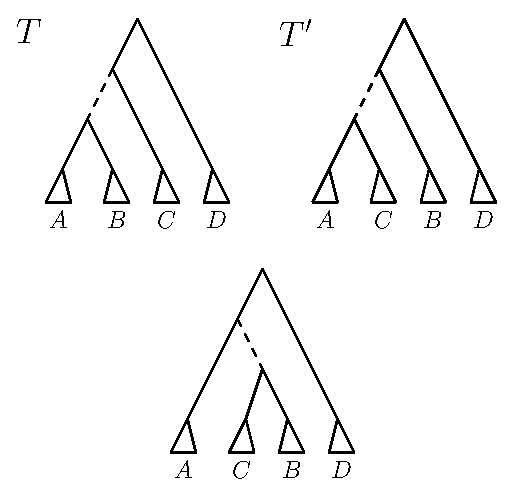
\includegraphics[width=0.4\textwidth]{thm_fp_nni1}
    \vspace{12pt}
    \caption{$\nni$ move between $T$ and $T'$ on the dashed edge $(v,w)$ and the third $\rnni$ neighbour resulting from a move on that edge.}
    \label{fig:thm_fp_nni1}
    \end{figure}

    \item $\nni$ moves on edge $(u,v)$ above $(v,w)$

    Notice that this is only possible if the interval above $(v,w)$ is an edge.
    As it is depicted in the top of Figure~\ref{fig:thm_fp_nni2a}, there are two $\nni$ moves on $(u,v)$ possible that lead to different trees.
    We stick to our notions of clusters $A,B,$ and $C$ as introduced above and additionally denote by $D$ the cluster induced by the child of $u$ that is not $v$.
    An illustration of this can be found in Figure~\ref{fig:thm_fp_nni2a}.

    \begin{figure}[H]
        \begin{subfigure}[b]{.45\textwidth}
            \centering
            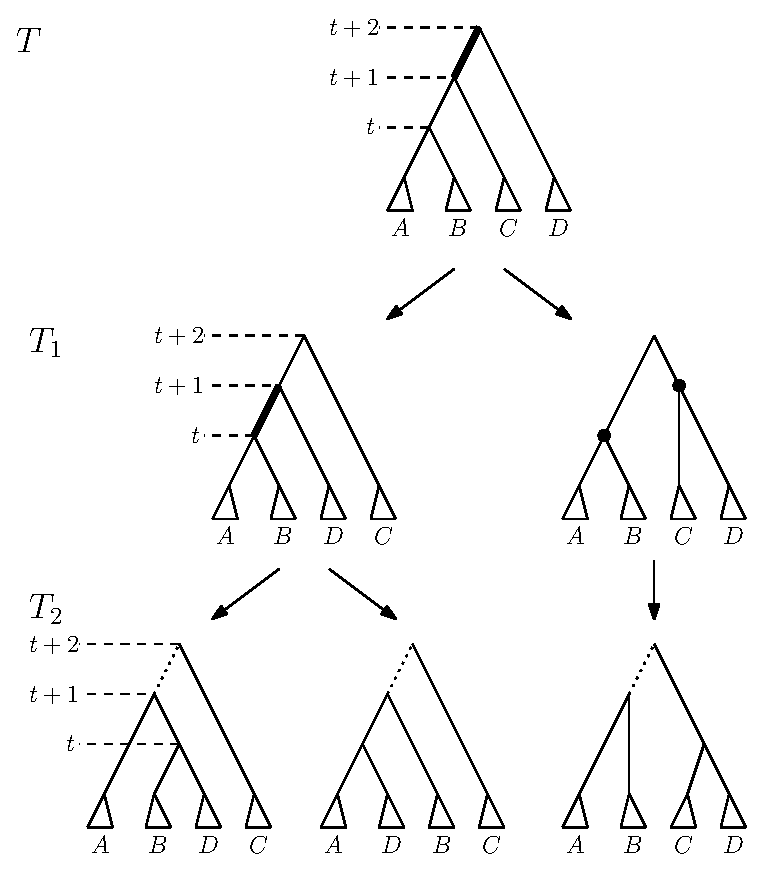
\includegraphics[width=0.9\linewidth]{thm_fp_nni2a.eps}
            \vspace{12pt}
            \caption{path $p$ following $T$}
            \label{fig:thm_fp_nni2a}
        \end{subfigure}
        \begin{subfigure}[b]{.45\textwidth}
            \centering
            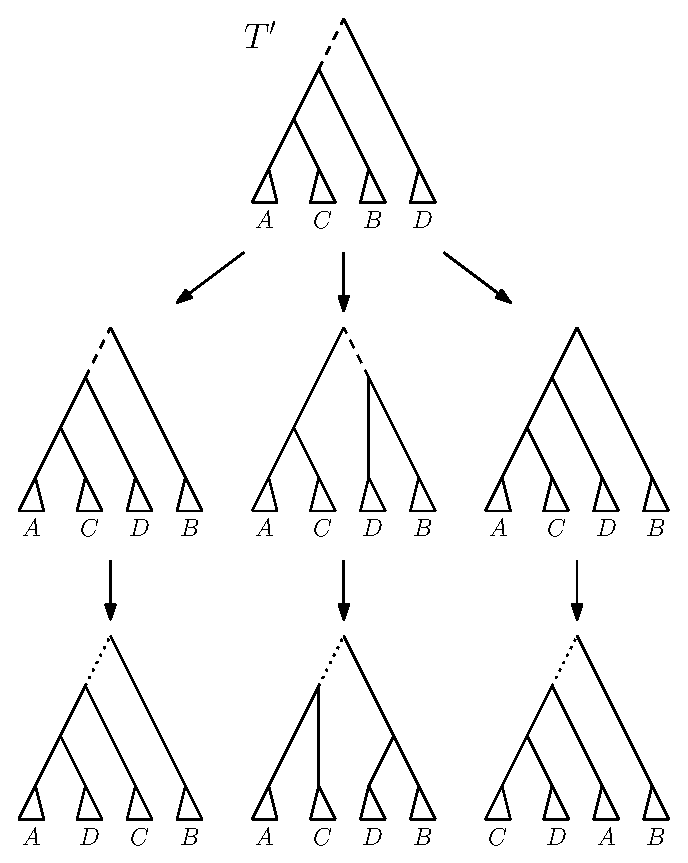
\includegraphics[width=0.9\linewidth]{thm_fp_nni2b.eps}
            \vspace{12pt}
            \caption{path $p'$ following $T'$}
            \label{fig:thm_fp_nni2b}
        \end{subfigure}
        \caption{Comparison of $p$ and $p'$ if there is an $\nni$ move on the edge $(u,v)$ above $(v,w)$ in $T$.
        The trees on the bottom are those following $T$ and $T'$ on $p$ and $p'$ after two $\rnni$ moves, respectively, depending on the cluster $C_k$ that is currently considered on $\findpath$:
        ${C_k \subseteq A \cup D}$ on the left, ${C_k \subseteq B \cup D}$ in the middle, ${C_k \subseteq C \cup D}$ on the right.}
    \end{figure}

    We will now consider each of the $\nni$ moves that are possible between $T$ and $\hat T$ separately.
    If $\hat T$ is the tree at the top left of Figure~\ref{fig:thm_fp_nni2a}, which results from $T$ by exchanging the subtrees induced by $C$ and $D$, the cluster $C_k$ that is moved down by $\findpath$ is either a subset of $A \cup B \cup D$, $A \cup D$ or $B \cup D$.

    \begin{enumerate}
        \item
        If $C_k \subseteq A \cup B \cup D$, then $C_k$ reached its final position in $\hat T$ on $p$.
            Specifically, it is $C_{k-1} = A \cup B$ in $T$ as $\findpath$ considers the cluster $C_1,\ldots C_{n-2}$ of $R$ in this order.
            It follows that on $p'$ there is a move that moves the most recent common ancestor of $C_{k-1} = A \cup B$ down right before $C_k$ is considered, again because $\findpath$ considers the cluster $C_{k-1}$ before cluster $C_k$.
            As a result the tree following $T'$ on $p'$ is $T$, contradicting $|FP(T',R)| < |FP(T,R)| - 1$.
        \item
            If $C_k \subseteq A \cup D$, the move on $\hat T$ on $p$ moves $(C_k)_{\hat T}$ further down by exchanging $B$ and $D$, resulting in a tree as depicted in the bottom left of Figure~\ref{fig:thm_fp_nni2a}.
            As the most recent common ancestor of the same cluster $C_k \subseteq A \cup D$ moves down on $p'$, the two moves following $T'$ exchange the subtree induce by $D$ down by exchanging it with its neighbours $B$ and $C$ as depicted on the left of Figure~\ref{fig:thm_fp_nni2b}.
            Comparing the trees on $p$ and $p'$ after the two moves following $T$ and $T'$, respectively, shows that we are again at a stage where two trees on these paths only differ by one edge (dotted edges in the trees at the bottom left of Figures~\ref{fig:thm_fp_nni2a} and~\ref{fig:thm_fp_nni2b}).
            Furthermore, the relation of the distances of these tree to $R$ are the same as the ones from $T$ and $T'$ to $R$, which contradicts the assumption that $T$ and $R$ are the closest pair of trees with this relation.
        \item
            If $C_k \subseteq B \cup D$, the two $\rnni$ moves following $T$ and $T'$ on $p$ and $p'$, respectively, end up in the trees depicted in the tree in the middle at the bottom of Figures~\ref{fig:thm_fp_nni2a} and \ref{fig:thm_fp_nni2b}, analogous to the previous case.
            As in the previous case, these trees coincide in all but one interval (dotted edges in the figure), which again contradicts the assumptions on $T$ and $R$.
    \end{enumerate}

    If the $\nni$ move on $(u,v)$ results in a tree $\hat T$ containing a subtree $C \cup D$ as illustrated on the top right of Figure~\ref{fig:thm_fp_nni2a}, it is $C_k \subseteq C \cup D$.
    If $(C_k)_T$ does not move further down on $p$, it follows that $C_k = A \cup B$ is a cluster in $R$ and that before $C_k$ is considered on $p'$, the most recent common ancestor of $C_{k-1} = (A \cup B)_{T'}$ moves down by one $\rnni$ move.
    Therefore $T$ follows $T'$ on $p'$, which contradicts $|FP(T',R)| < |FP(T,R)| - 1$.
    If on the other side the rank of $(C_k)_T$ decreases by more than one after tree $T$ on $p$, the move on $\hat T$ is a rank swap as depicted in the bottom right of Figure~\ref{fig:thm_fp_nni2a}.
    The moves on $p'$ that decreases the rank of $(C_k)_{T'}$ are $\nni$ moves exchanging $D$ with $B$ and $A$, because it is $C_k \subseteq C \cup D$.
    These moves are shown on the right of Figure~\ref{fig:thm_fp_nni2b}.
    As above, the two trees resulting from the two moves following $T$ and $T'$ on $p$ and $p'$, respectively, coincide by all but one interval.
    Therefore, we end up in the same contradiction as above.

    \item Rank move on interval $[u,v]$ above $(v,w)$

    Notice that this is only possible if $[u,v]$ is a rank interval.
    If after the rank move, which increases the rank of $v$, there is a rank move on $\hat T$ that increases the rank of $w$, the same rank moves happen on $p'$ and the trees after these two moves on $p$ and $p'$ coincide in all but one interval.
    As previously, this contradicts the assumption that $T$ and $R$ are the closest trees where there is a $T' \in N_1(T)$ with $|FP(T',R)| < |FP(T,R)| - 1$.
    If on the other side there is no such rank move on $\hat T$, then the cluster $C_{k-1} = A \cup B$ induced by $w$ is a cluster in $R$ as well.
    The tree following $T'$ on $p'$ is $T$ as it is the result of building this cluster in $T'$, which happens right before the cluster $C_k$ is being considered on $p'$.
    This is due to the order in which $\findpath$ considers most recent common ancestors of clusters.
    This contradicts $|FP(T',R)| < |FP(T,R)| - 1$.
    \todo{add a figure for this case}

    \item $\rnni$ moves on interval below $[v,w]$

    If there is a move on the interval below $[v,w]$, it is $C_k \subseteq A \cup B$.
    In this case, the move following $T'$ on $p'$ exchanges $B$ and $C$ by an $\nni$ move first, because this moves the most recent common ancestor of $C_k \subseteq A \cup B$ down.
    However, this transforms $T'$ into $T$, which contradicts $|FP(T',R)| < |FP(T,R)| - 1$.
\end{enumerate}

Let us now assume that there is a rank move between $T$ and $T'$ where nodes $v$ and $w$ inducing clusters $A$ and $B$ swap ranks as depicted at the top of Figure~\ref{fig:thm_fp_rank1}.
We will again consider the different moves from $T$ to $\hat T$ that are possible on intervals adjacent to $[v,w]$.

\begin{figure}[!hbt]
\centering
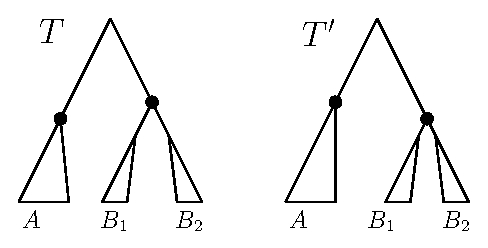
\includegraphics[width=0.4\textwidth]{thm_fp_rank1}
\vspace{12pt}
\caption{Rank move between $T$ and $T'$ on the interval given by the highlighted nodes, and an $\nni$ move on $T$ if the edge $(u,v)$ has length one.}
\label{fig:thm_fp_rank1}
\end{figure}

\begin{enumerate}
    \item Rank move on $[v,w]$

    The only possible move on $[v,w]$ on $T$ is a rank move resulting in $\hat T = T'$.
    It follows $|FP(T',R)| = |FP(T,R)| - 1$, which obviously contradicts our assumption $|FP(T',R)| < |FP(T,R)| - 1$.

    \item $\nni$ move on edge above $[v,w]$

    Notice that this is only possible if the interval above $[v,w]$ is an edge $(u,v)$ of length one.
    We are now going to distinguish the case that $u$ is the parent of $w$ from the case that it is not.
    At first we assume that $u$ is parent of $w$.
    It follows, that after the $\nni$ move on $(u,v)$, there is a new cluster containing $A$ and $B_1$, which is one of the subtrees that are children of $v$.
    This move is depicted on the left of Figure~\ref{fig:thm_fp_rank1}.
    If such a move happens the currently considered cluster $C_k$ must be subset of $A \cup B_1$, which means that $C_{k-1} = A$ is already at the same place in $T$ as in $R$.
    Therefore, the move on $p'$ on $T'$ must be a rank swap leading to $T$, as $(A)_{T'}$ is moved to its correct position before $C_k$ is considered, which follows from how $\findpath$ works.
    However, this means that $T$ is on the path $p'$ form $T'$ to $R$, which is a contradiction to $|FP(T',R)| < |FP(T,R)| - 1$

    Let us now assume that $u$ is not the parent of $w$.
    In this case the $\nni$ move builds a new cluster containing taxa of $B$ and of the cluster $C$ that is induced by the child of $u$ that is not $v$, as depicted in the top left of Figure~\ref{fig:thm_fp_rank2}.
    It follows that $C_k \subseteq C \cup B_1$ where $B_1$ is one of the clusters that is induced by a child of $w$.
    If there was no rank move on $\hat T$ decreasing the rank of $(C_k)_{\hat T}$ further, it must be $C_{k-1} = A$ meaning that $A$ is in the same position in $T$ as in $R$.
    In this case the tree following $T'$ on $p'$ is be $T$ as $C_{k-1} = A$ moves to it's final position on $\findpath$ before $C_k$ is moved down.
    However, this contradicts $|FP(T',R)| < |FP(T,R)| - 1$.
    Let us now consider what happens if there is a rank move on $\hat T$ that decreases the rank of $(C_k)_{\hat T}$ on $p$.
    This case is depicted on the left of Figure~\ref{fig:thm_fp_rank2}.
    The moves happening on $p'$ are as follows.
    As it is $C_k \subseteq C \cup B$, the rank of $(C_k)_{T'}$ decreases by a rank swap of $(C \cup B)_{T'}$ and $(A)_{T'}$ on $T'$ first and then an $\nni$ move exchanges $B_2$ and $C$, as it is depicted on the right in the same figure.
    One can easily see that the two trees on $p$ and $p'$ that are two $\rnni$ moves apart from $T$ and $T'$, respectively, only differ by one interval.
    Again, this is a contradiction to the fact that $T$ and $R$ are the trees with minimum distance for which we can find a $T' \in N_1(T)$ with $|FP(T',R)| < |FP(T,R)| - 1$.

    \begin{figure}[!hbt]
    \centering
    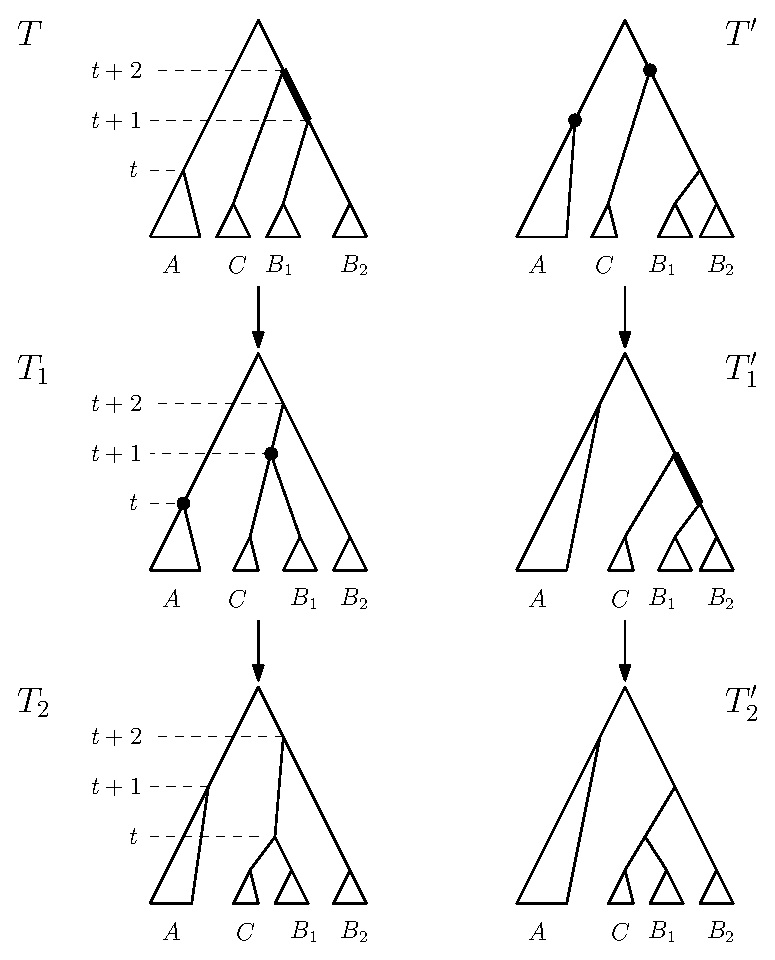
\includegraphics[width=0.4\textwidth]{thm_fp_rank2}
    \vspace{12pt}
    \caption{Comparison of $p$ (left) and $p'$ (right) if there is a rank move between $T$ and $T'$ and an $\nni$ move on the edge below the corresponding rank interval follows on $p$.}
    \label{fig:thm_fp_rank2}
    \end{figure}

    \item Rank move on interval above $[v,w]$

    Notice that this is only possible if the interval above $[v,w]$ is a rank interval.
    If there is a rank move increasing the rank of $v$, and no rank move increasing the rank of $w$ immediately afterwards, $C_k$ reaches it's final position in the tree $\hat T$ on $p$ following $T$.
    It follows that the cluster $A$ induced by $w$ in $T$ is the cluster $C_{k-1}$ in $R$.
    This means that the move following $T'$ on $p'$ leads to $T$, as the node inducing $A$ moves down before $C_k$ is considered on $\findpath$.
    This contradicts $|FP(T',R)| < |FP(T,R)| - 1$.
    If on the other side the rank swap on $T$ is directly followed by a rank swap increasing the rank of $w$, such rank swaps happen on $p'$ as well and the trees following $T$ and $T'$ after two $\rnni$ moves on $p$ and $p'$, respectively, coincide in all but one interval.
    This is again a contradiction to our choice of $T$ and $R$.

    \item $\rnni$ moves on interval below $[v,w]$

    If there is a move on the interval below $[v,w]$, it follows that $\findpath$ moves $C_k \subseteq A$ down where $A$ is the cluster induced by $w$.
    For decreasing the rank of the most recent common ancestor of $C_k \subseteq A$ in $T'$, the move on $T'$ must be a rank swap that results in $T$, contradicting  $|FP(T',R)| < |FP(T,R)| - 1$.
\end{enumerate}

We can conclude that in any of the above cases we end up in a contradiction, proving that a tree $T'$ with $|FP(T',R)| < |FP(T,R)| - 1$ does not exist in $N_1(T)$.
Therefore we can follow that $|FP(T',R)| \geq |FP(T,R)| -1$ for all $T' \in N_1(T)$.
\endproof

\end{document}
